\documentclass{standalone}
\usepackage{tikz}
\usepackage{fontspec}

\definecolor{eins}{HTML}{e7e7e8}   %% Ring 1 "core"     - weiß - Mittelpunkt, Ring um Mittelpunkt
\definecolor{zwei}{HTML}{ed1c24}   %% Ring 2 "com"      - rot -  "Fenster" innen
\definecolor{drei}{HTML}{fbad18}   %% Ring 3  "culture" - orange - fünf Module, quasi invertiert
\definecolor{vier}{HTML}{74c043}   %% Ring 4  "creactiv" - grün -  vier Module
\definecolor{fuenf}{HTML}{0089d0}  %% Ring 5 "cience"  - cyan (blau) - drei Module mit "Strich"
\definecolor{sechs}{HTML}{11357e}  %% Ring 6 "carbon" -  indigo - viele "Fenster" außen
\definecolor{sieben}{HTML}{000000} %% Ring 7 "clamp" -  schwarz, c-förmig
\definecolor{cbase}{HTML}{222222}  %% Körper der Raumstation    

\newcommand{\ceva}[1]{ {\fontspec{[ceva-c2.ttf]}#1}}
\newcommand{\cevain}[1]{{ \fontspec{[ceva-c2.ttf]}#1} | \emph{#1}}

\begin{document}
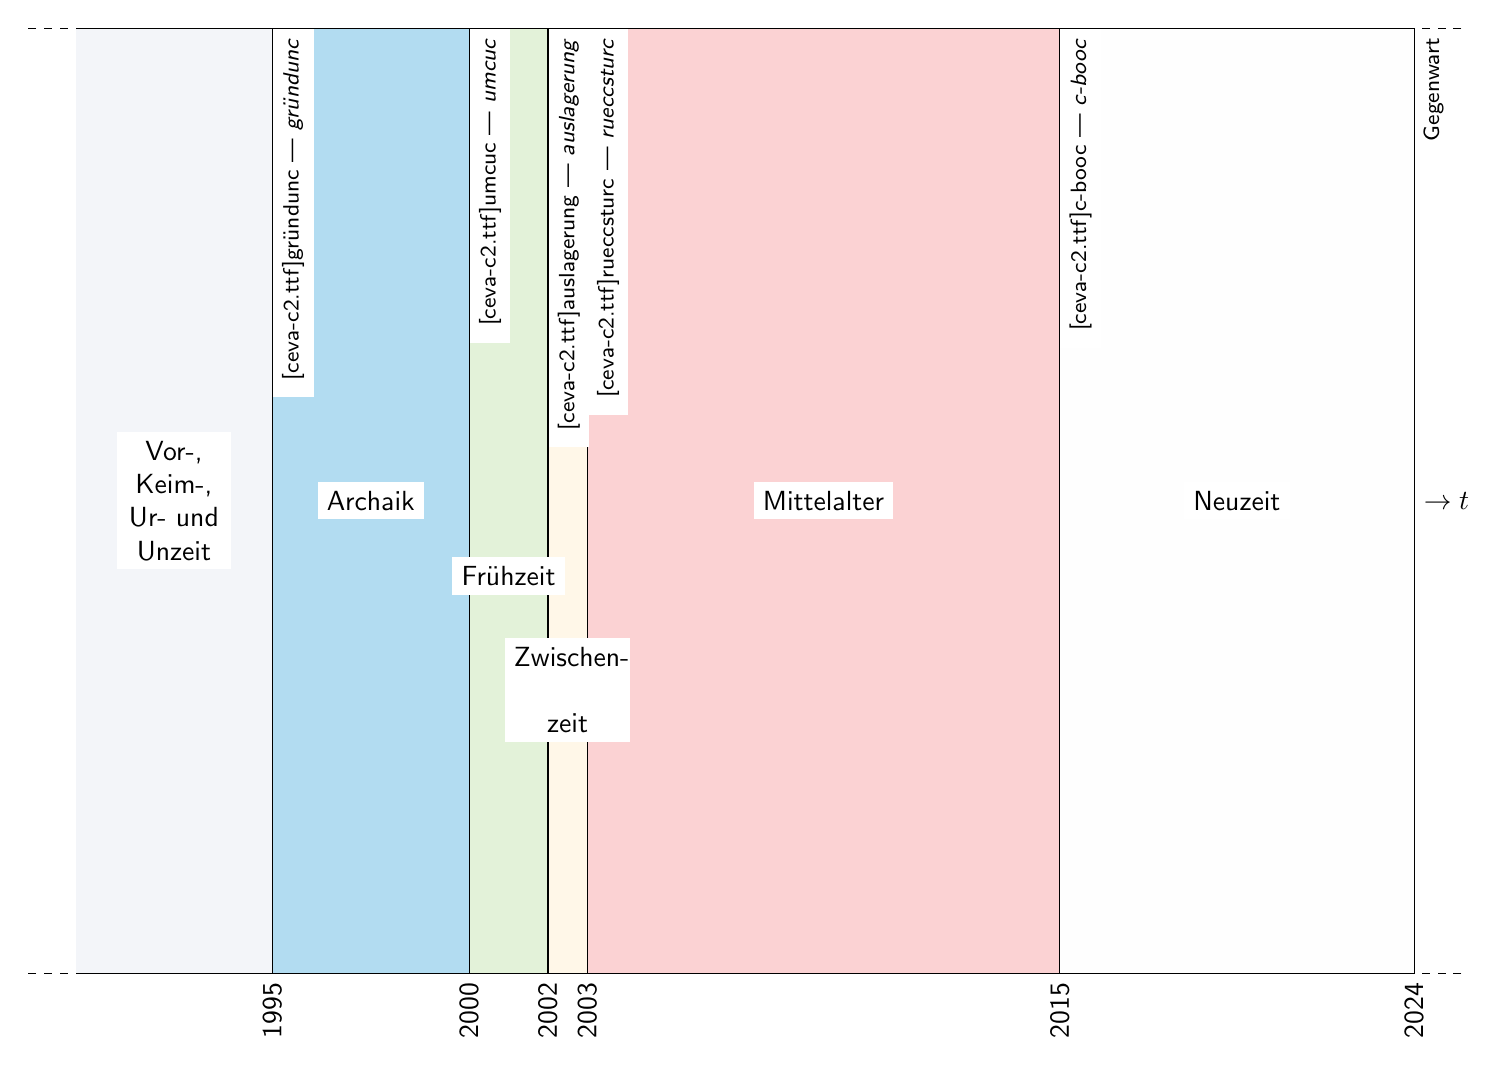
\begin{tikzpicture}[yscale=2.4,xscale=-0.5,rotate=90,
    every node/.style={
        fill=white,font=\sffamily 
        }
    ]
    % \draw (0) rectangle (0,,1);
    \foreach \i in {124.4,124.8,125.2} 
        {
        \draw (0,\i) -- (0,\i-0.2);
        \draw (5,\i) -- (5,\i-0.2);
        }

    \node [right] at (2.5,124) {$\rightarrow t$  };
    
    \node [below left,rotate=90] at (5,124) {\footnotesize Gegenwart};
    
    \draw[fill=eins!5] (0,124) node [left, rotate=90]{2024} rectangle node {Neuzeit} (5,115) node [below left,rotate=90] {\footnotesize\cevain{c-booc}};
    % \draw (0,115) -- (0,124); draw (5,114) -- (5,124); \draw (0,115
    
    \draw[fill=zwei!20] (0,115) node [left, rotate=90]{2015} rectangle node {Mittelalter} (5,103) node [below left,rotate=90] {\footnotesize\cevain{rueccsturc}};
    
    \draw[fill=drei!10] (0,103)  node [left, rotate=90]{2003} rectangle   (5,102) node [below left,rotate=90] {\footnotesize\cevain{auslagerung}};
    
    \draw[fill=vier!20] (0,102)  node [left, rotate=90]{2002} rectangle (5,100) node [below left,rotate=90] {\footnotesize\cevain{umcuc}};

    
    \draw[fill=fuenf!30] (0,100)  node [left, rotate=90]{2000} rectangle node {Archaik} (5,95) node [below left,rotate=90]{\footnotesize\cevain{gründunc}};
    % \node at (0,95) [left] {1995};
    
    \draw[fill=sechs!5,draw=none] (0,95)  node [left, rotate=90]{1995} rectangle node[text width=8ex,align=center] {Vor-, Keim-, Ur- und Unzeit} (5,90) ;
    \draw (0,95) -- (0,90); \draw (5,95) -- (5,90);
    
    \foreach \i in {89.8,89.4,89} 
        {
        \draw (0,\i) -- (0,\i-0.2);
        \draw (5,\i) -- (5,\i-0.2);
        }

    \node at (2.1,101) {Frühzeit};
    \node [text width=9ex, align=center] at (1.5,102.5) {Zwischen-\\zeit};
    
    % \draw[<->] (0,95) rectangle (0,65);
\end{tikzpicture}

\end{document}
